\documentclass[../main.tex]{subfiles}

\begin{document}

\section{Optimal Control of Pitch/Travel without Feedback}\label{kap:Part2OptimalControlWithoutFeedback}

\subsection{Derivation of a continous time state space model}
In this part of the exercise we will disregard elevation, therefore we assume $ e = 0 $ and do include it in the model.

The state-vector, $\bm x$ is defined as:
\begin{equation}\label{eq:lab2_state}
	\bm x = 
	\begin{bmatrix}
		\lambda & r & p & \dot p
	\end{bmatrix}
	^T ,
\end{equation}
where $\lambda$ is travel, $r$ is the travel rate, $p$ is pitch and $\dot{p}$ is pitch rate.

The dynamic equations for the system was given in the problem description \todo{Add ref to page and paper}. These following equations were given:
\begin{subequations} \label{eq:lab2_states_eq}
	\begin{align}
		\dot \lambda &= r \\
		\dot r &= -K_2 p, \quad K_2 = \frac{K_p l_a}{J_t}\\
		\dot p &= \dot p \\
		\ddot p &= -K_1 V_d = K_1 K_{pd} \dot p - K_1 K_{pp} p + K_1 K_{pp} pc, \quad K_1 = \frac{K_f l_h}{J_p}
	\end{align}
\end{subequations}
The state-space form of the system therefore becomes: 
\begin{equation}\label{eq:lab2_cont_ss}
	\underbrace{\begin{bmatrix}
		\dot \lambda \\
		\dot r \\
		\dot p \\
		\ddot p
	\end{bmatrix}}_{\bm{\dot x}} = 
	\underbrace{
	\begin{bmatrix}
		0 & 1 & 0 & 0 \\
		0 & 0 & -K_2 & 0 \\
		0 & 0 & 0 & 1 \\
		0 & 0 & -K_1 K_{pp} &  -K_1 K_{pd}
	\end{bmatrix}
	}_{\bm A_c}
	\begin{bmatrix}
		\lambda \\ r \\ p \\ \dot{p} \\
	\end{bmatrix}
	+
	\underbrace{
		\begin{bmatrix}
			0 \\ 0 \\ 0 \\ K_1 K_{pp}
		\end{bmatrix}
	}_{\bm B_c} \underbrace{p_c}_{u}
\end{equation}

\subsubsection{A deeper dive into the state-space model}
The state-space form of the system models two part of the whole system, namely: 
\begin{enumerate}
	\item The physics of the helicopter.
	\item The proportional-derivative controller for the pitch.
\end{enumerate}
This is shown in \cref{fig:lab2_system} where the red dotted box shows what we model with the state space model. \todo[inline]{Add ref to the figure in the problem description}

\begin{figure}[h]
	\centering
	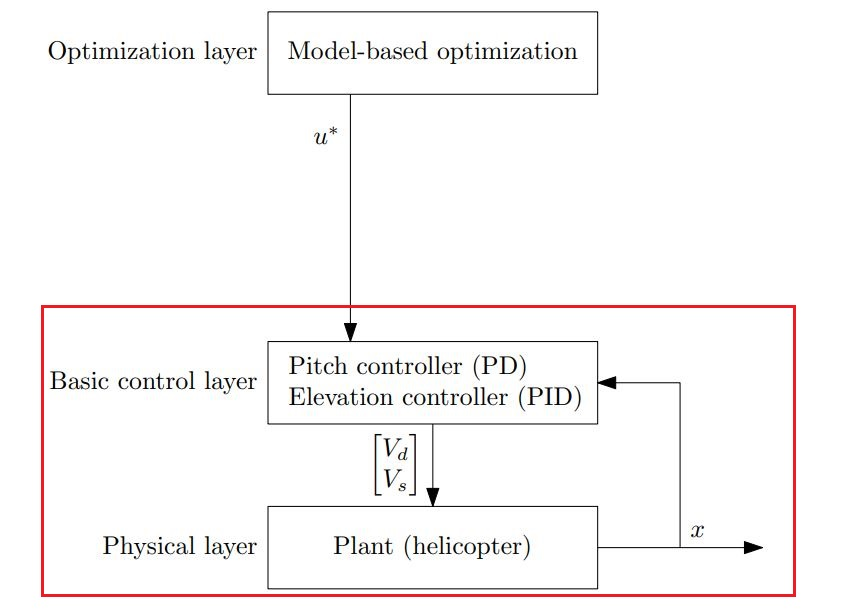
\includegraphics[width=0.8\linewidth]{figures/lab2_system}
	\caption{The red box encapsulate what is modelled in the state space model described by \cref{eq:lab2_cont_ss}.}
	\label{fig:lab2_system}
\end{figure}

This becomes clear studying the equations in \cref{eq:lab2_states_eq}. They describe the helicopters physics for all states except elevation and elevation rate. $ \lambda $ and $ r $ is dependent on the helicopters pitch, $ p $. $ p $ and $ \dot p  $ is however dependent on the voltage difference, $ V_d $. The voltage difference is the output of the PD-controller for controlling the pitch\todo{Should we add acronym list?}. 

To summarize, this means that our state space model describes the helicopter's physics through the dynamic equations for $ \lambda $, $ r $, $ p $ and $ \dot p $, while the equation of $ V_d $ describes the PD-controller used to control the pitch angle. In total our state-space model is modelling both the helicopter and the PD controller for pitch.


\subsubsection{Stability and eigenvalues}
The properties of this system is dependent on physical constants ($l_a, J_t, ...$) and control parameters ($K_{pp}, K_{pd}$).

Symbolic expressions in Matlab shows that the eigenvalues of A are:
\begin{equation}
	\lambda = \pm \frac{1}{2} \left( \sqrt{-K_1 (-K_1 K_{pd}^2 + 4  K_{pp})} - K_1  K_{pd} \right)
\end{equation}

The eigenvalues of the continous model, with $K_{pp} = 0,1 , K_{pd} = 0,4$ are:
\begin{equation}\label{eq:lab2_ss_c_eigenvalues_example}
	\begin{bmatrix}
		0 \\ 0 \\ -0.26 + 0.24i \\ -0.26 - 0.24 \\
	\end{bmatrix}
\end{equation}

% ------------------- DISCRETIZING THE MODEL ------------------------
\subsection{Discretizing the continous time model}
A discretized model is required for generating an optimal trajectory. \textit{[...] continous time models require quite different solution methods} \cite{FossHeirung}

We will discretize the model using the forward Euler method, which is given by:
\todo[inline]{Do we need to derive forward euler?}
\begin{equation}\label{eq:lab2_forward_euler}
	\bm{x}[k + 1] = \bm I \bm x[k] + T\bm{A_c x}[k] + T\bm B_c ,
\end{equation}
where $ T $ is the sample-time in the discrete model.\todo
[inline]{Add reference to linsys slides}
Reformulating this, we can write:
\begin{equation}\label{eq:lab2_discrete_system}
	\bm{x}_{k + 1} = \underbrace{(\bm I + T \bm A_c)}_{\bm A_d} \bm{x}_{k} + \underbrace{T \bm B_c}_{\bm B_d} u_k
\end{equation}
On matrix form $ \bm A_d $ and $ \bm B_d $ becomes: 
\begin{equation}
	\bm A_d = \begin{bmatrix}
		1 & T & 0 & 0 \\
		0 & 1 & -T K_2 & 0 \\
		0 & 0 & 1 & T \\
		0 & 0 & -T K_1 K_{pp} &  1 - T K_1 K_{pd}
	\end{bmatrix}, \quad 
	\bm B_d = \begin{bmatrix}
		0 \\ 0 \\ 0 \\T K_1 K_{pp}
	\end{bmatrix}
\end{equation}




\subsubsection{Checking stability}
The stability condition for \cref{eq:lab2_discrete_system} is that all eigenvalues of $ \bm A_d $ is less than one in absolute values, i.e.:
\begin{equation}\label{eq:lab2_stab_condition}
	|\lambda_i| \leq 1, \quad \text{for } i = 1, 2, 3, 4
\end{equation}, where $ \lambda_i $ is the i'th eigenvalue of $ \bm A_d $.

Using the script in \cref{lst:lab2_eigenvalues} the eigenvalues became:
\begin{subequations}\label{eq:lab2_eigenvalues}
	\begin{align}
		\lambda_1 &= 1 \\
		\lambda_2 &= 1 \\
		\lambda_3 &= 0.55 \\
		\lambda_4 &= 0.55
	\end{align}
\end{subequations}
All eigenvalues fulfills the requirement of \cref{eq:lab2_stab_condition}, which means our system is stable! Since two of the eigenvalues are on the unit circle (i.e. has a value of 1), our system is more specifically marginally stable. More information on this subject can be found \todo{Add cite to wikipedia}.

\lstinputlisting[caption= {MATLAB code for calculating eigenvalues for $ \bm A_d $}, label = {lst:lab2_eigenvalues}, language=Matlab]{code/calculate_eigenvals.m}

\subsection{The open loop optimization problem}
% https://ntnu.blackboard.com/ultra/courses/_24653_1/cl/outline
%where $q$ is the weight of input-usage. Subject to constraints.
The open loop optimization problem is a constrained quadratic program that can be solved using the Matlab function quadprog. The quadprog function requires the input to be in standard form:

\begin{equation}\label{eq:lab2_quadprog_std_form}
	\min_x \frac{1}{2} \bm x^t \bm H \bm x + \bm f^T \bm x \quad \text{such that} \begin{cases}
		\bm A \bm x \leq \bm b, \\
		\bm A_{eq} \bm x = \bm B_{eq}, \\
		\bm{lb} \leq \bm x \leq \bm{ub}		
	\end{cases}
\end{equation}

The next subsections describes this process.

\subsubsection{Formulating the cost function} \label{sec:lab2_cost_func}
As the problem description states, the cost function used in this exercise is:
\begin{equation} \label{eq:lab2_start_cost_func}
	\phi = \sum_{i=0}^{N-1} \left( \lambda_{i+1} - \lambda_f \right)^2 + qp_{ci}^2 , \quad q \ge 0
\end{equation}

Which can be rewritten with $ \bm x $ and $ u $:
\begin{equation}\label{eq:lab2_start_cost_func_2}
	f(\bm x, u) = \sum_{i=0}^{N-1} \left( \bm x_{i+1} - \bm x_f \right)^T \bm Q \left( \bm x_{i+1} - \bm x_f \right) + q u^2
\end{equation}
where
\begin{equation}\label{eq:lab2_lambda_f}
	\bm x_f = \begin{bmatrix}
		\lambda_f \\ 0 \\ 0 \\ 0
	\end{bmatrix}
\end{equation}
\begin{equation}\label{eq:lab2_Q}
	\bm Q = \begin{bmatrix}
		1 & 0 & 0 & 0 \\
		0 & 0 & 0 & 0 \\
		0 & 0 & 0 & 0 \\
		0 & 0 & 0 & 0
	\end{bmatrix}
\end{equation}
In this case we have that $ \lambda_f = 0 $ and therefore $ \bm x_f = \bm 0 $, and \cref{eq:lab2_start_cost_func_2} can be rewritten as:

\begin{equation}\label{eq:lab2_LQR}
	f(\bm x, u) = \sum_{i=0}^{N-1} \bm x_{i+1}^T \bm Q \bm x_{i+1} + r u^2
\end{equation}
where
\begin{equation}\label{eq:lab2_R}
	r = q
\end{equation}

This summation form can be rewritten into matrix form by using the $z$ vector:
\begin{equation}\label{eq:lab2_z}
	\bm z = \begin{bmatrix}
		\bm x_1 & \bm x_2 & ... & \bm x_n & u_0 & u_1 &... & u_{n-1} 
	\end{bmatrix}^T
\end{equation}

Into the standard quadratic form:
\begin{equation}\label{eq:lab2_quadprog}
	f(\bm z) = \bm z^T \bm H \bm z
\end{equation}
with
\begin{equation}\label{eq:lab2_H}
	\bm H = \begin{bmatrix}
		\bm Q & 0 & \cdots  & 0 & 0 & 0 & \cdots & 0\\
		0 & \bm Q & \cdots  & 0 & 0 & 0 & \cdots & 0\\
		 & & \ddots &  &  &  &  & \\
		0 & 0 & \cdots & \bm Q & 0 & 0  & \cdots & 0\\
		0 & 0 & \cdots & 0 & r & 0  & \cdots & 0\\
		0 & 0 & \cdots & 0 & 0 & r  & \cdots & 0\\
		 & &  &  &  &  & \ddots & \\
		0 & 0 & \cdots & 0 & 0 & 0  & \cdots & r
	\end{bmatrix}
\end{equation}


\subsubsection{The constraints of the optimization problem} \label{sec:lab2_constraints}
There are two separate types of constrains in this problem, the system itself and imposed constraints. The system constrains is described by the physics of the helicopter, which we have modeled in \cref{eq:lab2_discrete_system}. Imposed constraints are constraints added by the designer of the system. 

In this case we have an imposed constraint on the pitch given by:
\begin{equation}
	\left\lvert p_k \right\rvert \le \frac{30}{180} \pi, k \in \left\{ 1, ..., N \right\} 
\end{equation}
As the manipulated variable $ p_c $ is the setpoint for the $ p $ controller, this constraint must also be implemented for the setpoint. Since there is no inequality constraints on the other states, they have lower bounds of $ -\infty $ and upper bounds of $ \infty $. This gives us the inequality constraints for the state and the input as: 
\begin{subequations}
	\begin{align}
		\bm x^{low} = \begin{bmatrix}-\infty \\ -\infty \\ -\frac{30}{180} \pi \\ -\infty \end{bmatrix} &\leq \bm x \leq \bm x^{high} = \begin{bmatrix} \infty \\ \infty \\ \frac{30}{180} \pi \\ \infty \end{bmatrix} \\
		u^{low} = -\frac{30}{180} \pi &\leq u \leq u^{high} = -\frac{30}{180} \pi
	\end{align}
\end{subequations}
We can now easily expand this to define lower- and upper-bounds for the vector $ \bm z $ given in \cref{eq:lab2_z}
\begin{equation}\label{eq:lab2_z_bounds}
		\bm z^{low} = \begin{bmatrix}
			\bm x^{low}\\
			\vdots \\
			\bm x^{low}\\
			u^{low}\\
			\vdots \\
			u^{low}
		\end{bmatrix} \leq \bm z \leq
		\bm z^{high} = \begin{bmatrix}
			\bm x^{high}\\
			\vdots\\
			\bm x^{high}\\
			u^{high}\\
			\vdots \\
			u^{high}\\
		\end{bmatrix}
\end{equation}



The system constraints can be defined as: 
\begin{equation}\label{eq:lab2_physical_constraints}
	\bm A_{eq} \bm z = \bm b_{eq}
\end{equation}
, where
%The physics of the helicopter is added in $A_{eq}$ and $b_{eq}$.
\begin{equation} \label{eq:lab2_Aeq_beq}
	\bm A_{eq} = 
	\begin{bmatrix}
		\bm I & 0 & \cdots & \cdots & 0 & -\bm B_d & 0 & \cdots & \cdots & 0 \\
		-\bm A_d & \bm I & \ddots & & \vdots & 0 & \ddots & \ddots & & \vdots \\
		\vdots && \ddots & \ddots & 0 & \vdots & & \ddots & \ddots & 0 \\
		0 & \cdots & 0 & -\bm A_d & \bm I & 0 & \cdots & \cdots & 0 & -\bm B_d
	\end{bmatrix}, \; 
	\bm b_{eq} =
	\begin{bmatrix}
		\bm A_d \bm x_0 \\ 0 \\ \vdots \\ 0
	\end{bmatrix}
\end{equation}

Performing the multiplication (and abusing notation) shows that:
\begin{equation} \label{eq:lab2_system_constraints}
	\bm A_{eq} \bm z = \bm b_{eq} \implies
	\begin{bmatrix}
		\bm x_1-\bm B_d u_0 = \bm A_d \bm x_0 \\
		-\bm A_d \bm x_1 + \bm x_2 - \bm B_d u_1 = 0 \\
		\vdots \\
		-\bm A_d \bm x_{n-1} + \bm x_n - \bm B_d u_{n-1} = 0 \\
	\end{bmatrix} \implies
	\begin{bmatrix}
		\bm x_1 = \bm A_d \bm x_0 + \bm B_d u_0 \\
		\bm x_2 = \bm A_d \bm x_1 + \bm B_d u_1 \\
	 	\vdots \\
		\bm x_n = \bm A_d \bm x_{n-1} + \bm B_d u_{n-1}
	\end{bmatrix}
\end{equation}
\Cref{eq:lab2_system_constraints} describes the system in terms of \cref{eq:lab2_discrete_system} for all timesteps\todo{Again: timesteps illegal?}, and thereby also describes all system constraints for the system.

\subsubsection{Defining the open loop optimization problem}
Combining the cost function described in \cref{sec:lab2_cost_func} and the constraints described in \cref{sec:lab2_constraints} the open loop optimization problem can be defined as: 

\begin{equation}\label{eq:lab2_open_loop_opt_problem}
	f(\bm z) = \bm z^T \bm  H \bm z \quad \text{s.t.} \quad 
	\begin{cases}
		\bm A_{eq} \bm z = \bm B_{eq} \\
		\bm z^{low} \leq \bm z \leq \bm z^{high}
	\end{cases} 
\end{equation}, 
where $ \bm z $ is given by \cref{eq:lab2_z}, $ \bm H $ is given by \cref{eq:lab2_H}, $ \bm A_{eq} $ and $ \bm B_{eq} $ is given by \cref{eq:lab2_Aeq_beq}, and $ \bm z_{low} $ and $ \bm z_{high} $ is given by \cref{eq:lab2_z_bounds}.

It is now easy to compare this to the QP formulation given in \cref{eq:lab2_quadprog_std_form}, and implement this in MATLAB. This is done in \cref{lst:lab2_matlab}. 

\textbf{NB:} that the variable names are not exactly the same in the code as in the sections above, but the procedure is the same.

\subsection{The weights of the optimization problem}
\textit{Try using the values 0.1, 1 and 10 as weights q. Plot the manipulated variable and the output. Comment the results with respect to the different weights chosen.}

$ \bm Q $ and $ r $ in \cref{eq:lab2_LQR} are typically called weight-matrices. Their relative values reflect how the LQ regulator prioritize the objectives (the state and the input) relative ot each other. In this problem, $ \bm Q $ is kept constant and the group changed the value of $ r $ (or $ q $ as it is called in the problem description). Increasing the value of $ q $ means that we are placing a higher cost of input - reducing the input usage. In other words, a smaller $ q $ will make the ``fuel'' (or input) expensive. 
%This will in turn mean that the cost of deviation in $\lambda$ is, in relation to the input, cheaper. 
The result is lower input usage and a slower response. This is exactly what is seen in \cref{fig:lab2_optimalu}.

\begin{figure}[h]
	\centering
	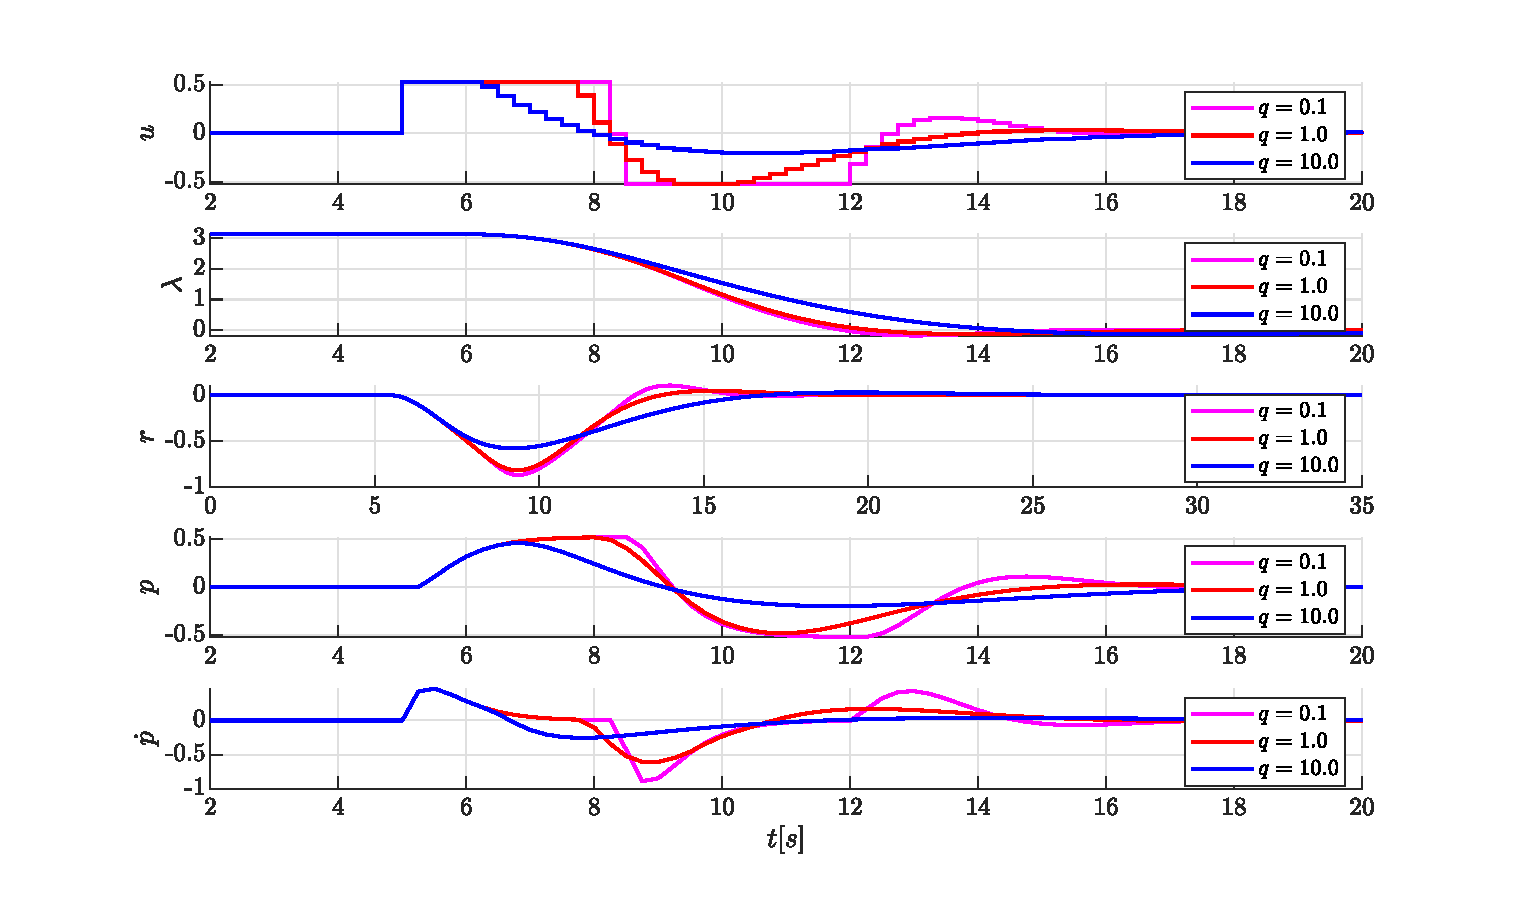
\includegraphics[width=\linewidth]{figures/lab2_optimal_u}
	\caption{Optimal trajectories for the manipulated variable and outputs with different values of $q$.}
	\label{fig:lab2_optimalu}
\end{figure}

\Cref{fig:lab2_optimalu} also shows how the constraints work in practice. Studying the plot of $ u $, we can see that no matter how low $ q $ is, the input never goes beyond the specified range of $ \pm\frac{30}{180} \pi $.

\subsection{The objective function}
\textit{Furthermore, discuss the objective function (15) (in the lab assignment text) in particular the term $(\lambda_i-\lambda_f )^2$. For instance, could any unwanted effects arise from steering the helicopter to $\lambda =\lambda_f$ with this objective function?}

The term $(\lambda_i-\lambda_f )^2$ in \cref{eq:lab2_start_cost_func} may cause problems if it becomes too large compared to the term $ q \cdot u^2 $. What is meant by ``too large'' is that the solution will actually never reach $ \lambda_f $ in the given time horizon, because it is theoretically impossible due to the problem constraints. \Cref{fig:lab2_too_large} shows this. This is the solution of the optimization problem when the group used $ \lambda_0 = 40\pi $. It shows that when the error term for the travel is too large, the helicopter will never reach $ \lambda_f $ no matter what. A direct consequence of this is that the helicopter will never stop the rotation before the time horizon ends.
\begin{figure}[h]
	\centering
	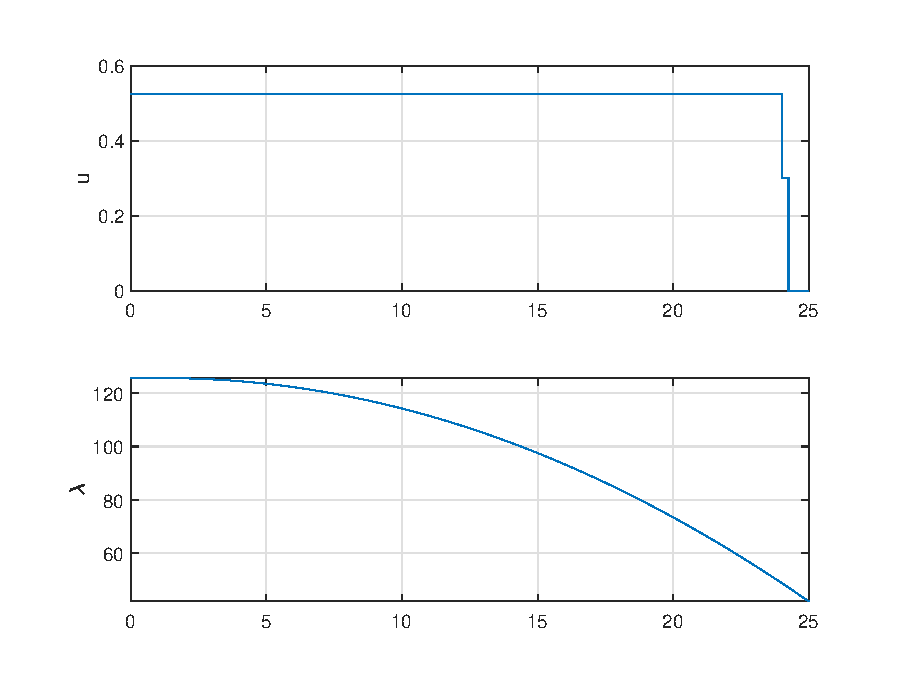
\includegraphics[width=\linewidth]{figures/lab2_1_5_example.eps}
	\caption{Optimal trajectories using $\lambda_0 = 40\pi$ .}
	\label{fig:lab2_too_large}
\end{figure}
\Cref{fig:lab2_too_large} also shows that increasing $(\lambda_i-\lambda_f )^2$ has the same effect as increasing $ \bm Q $ relative to $ r $ in \cref{eq:lab2_LQR}; it will prioritize to minimize $(\lambda_i-\lambda_f )^2$ and use much input to achieve this. We say that the ``fuel'' is cheap.

The ``solution'' to this problem is to increase the time horizon either by adding more steps (increase $N$) or increase the sampling time. This will give the optimization problem enough time to reach the $ \lambda_f $. This is shown in \cref{fig:lab2_inc_delta_t}. In this case the sampling time was doubled from $ 0.25 $ to $ 0.5 $, and the optimization problem had almost enough time to stop rotating at the final value. 
\begin{figure}[h]
	\centering
	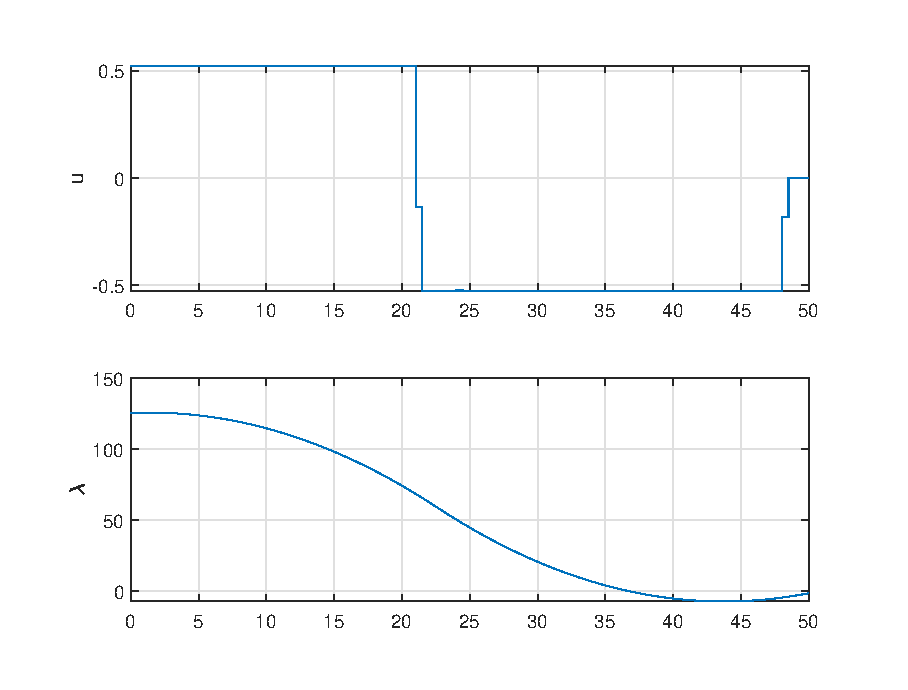
\includegraphics[width=\linewidth]{figures/lab2_1_5_example_2.eps}
	\caption{Optimal trajectories using $\lambda_0 = 40\pi$ and $ \Delta t = 0.5$ .}
	\label{fig:lab2_inc_delta_t}
\end{figure}

\subsubsection{Improved $ \lambda_0 $ selection}
In the case of the lab setup, it does not really make any sense to have $ \lambda_i-\lambda_f >  2\pi $, because the helicopter is always on a circles edge. The result of this is that $ \lambda = 0 $, $ \lambda = 2\pi $ and $ \lambda = 4\pi $ and so on, is essentially the same helicopter-configuration. 

Also, the way the objective function is set up, it will not choose the always choose the shortest way to $ \lambda_f $. If $ \lambda_0 = \frac{3}{4} \pi $, this means that the helicopter is $\frac{3}{4} \pi $ radians from $ \lambda_f $ in the counter-clockwise direction and  $\frac{1}{4} \pi $ radians from  $ \lambda_f $ in the clockwise direction. Therefore, it is most logical to go the clockwise direction, because this requires the least amount of input. However, the way the objective function is chosen, it will go in the counter-clockwise direction.

Therefore, a suggested solution from the group, is to use the following formula for $ \lambda_0 $: 
\begin{subequations}
	\begin{align}
		\lambda_{0, \text{modified}} &= \begin{cases}
			+\text{mod}(\lambda_0-\lambda_f, 2\pi), \quad &\text{if} \quad \text{mod}(\lambda_0-\lambda_f, 2\pi) \leq \pi \\
			-(2 \pi - \text{mod}(\lambda_0-\lambda_f, 2\pi)) \quad &\text{else}
		\end{cases} \\ 
	\end{align}
\end{subequations}, where $ \text{mod} $ is the modulus operator.

This will insure that $ \lambda_i-\lambda_f \leq  2\pi $ for all $ i \in (0, 1, 2, ..., N-1) $ and it will also insure that the helicopter will choose the shortest direction.

It is easily implemented in the code, as \cref{lst:improved_lambda_0} shows.
\begin{lstlisting} [caption={Improved $\lambda_0$ implementation.}, label={lst:improved_lambda_0}]
	lambda_0 = 4/3*pi; %Some value
	lambda_0 = mod(lambda_0, 2*pi);
	if (lambda_0 > pi)
		lambda_0 = -(2*pi - lambda_0);
	end
\end{lstlisting} 

\clearpage
\subsection{Experimental results}\label{kap:task_10_2_experimental_results}
The group performed two experiments with the helicopter:
\begin{enumerate}
	\item Flight with optimal setpoints: $u_k = u_k^*$
	\item Flight without setpoints: $u_k = 0$
\end{enumerate}
Both fligths, along with the optimal trajectory and a compensated trajectory are plotted in \cref{fig:LAB2_plot_1}.

\begin{figure}[h]
	\centering
	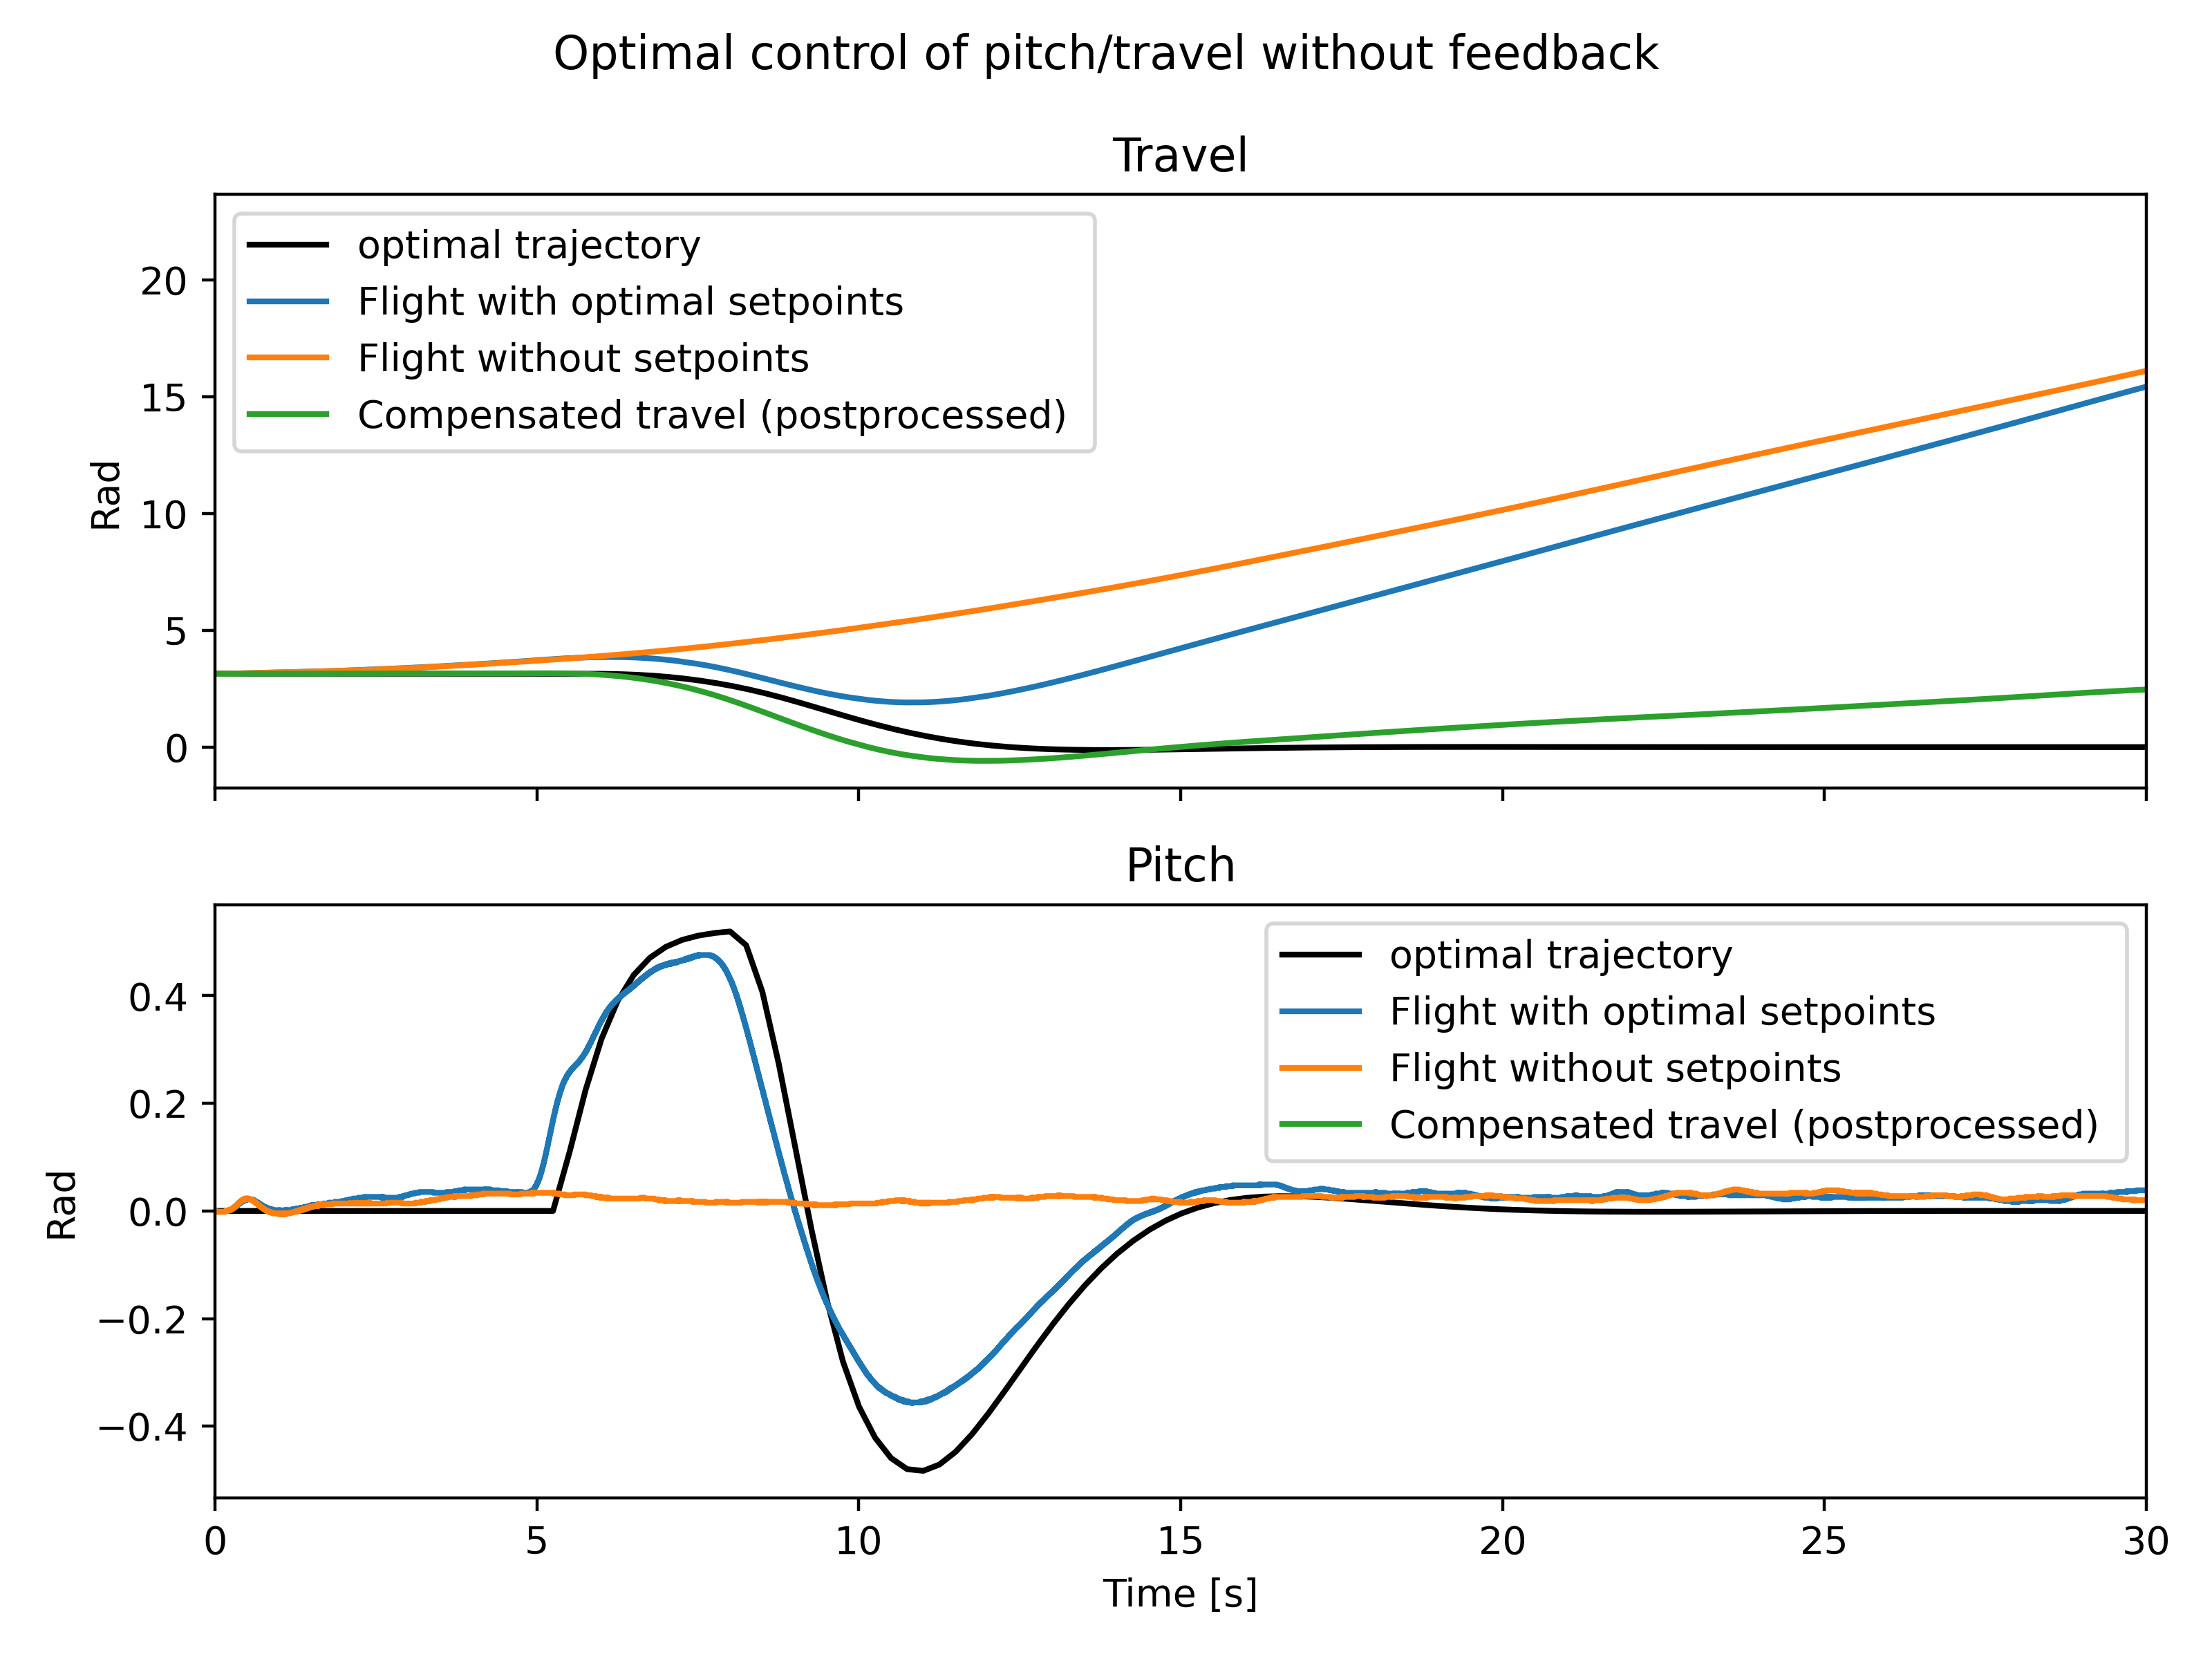
\includegraphics[width=0.8\linewidth]{figures/LAB2_plot_1.png}
	\caption{Results of LAB2}
	\label{fig:LAB2_plot_1}
\end{figure}

\subsubsection{Pitch-control}
It is clear that both fligths have adequate control of pitch. In the case where $u_k = 0$ the pitch is close to $0$. In the case where $u_k = u_k^*$ the pitch is close to the optimal trajectory.

This is expected as pitch-control is a closed loop - the basic control layer has a PD controller that ensures that pitch follows the reference $u_k$.

\subsubsection{Travel-drift}\label{kap:LAB2_travel_drift_causes}
From the flight with $u_k = 0$ it is clear that there is significant travel-drift present in the helicopter. Even when pitch is very close to $0$ the helicopter travels quickly far away from the initial point.

There are three main causes of drift:
\begin{enumerate}
	\item The encoder-measurement of pitch is not precise
	\item Helicopter inbalance
	\item Disturbances
\end{enumerate}

When the helicopter starts, it reads the initial \textbf{encoder}-value for the pitch, and assumes this is equal to zero. However, if the platform is not built precisely, the encoder axis may not be 100 \% aligned with the corresponding real world axis. There are many possible reasons for this, but it will not be discussed further. Regardless of the cause, the effect will be the same: The measured encoder-value will have a constant offset compared to real world-values. This will again cause the helicopter to drift when it measures zero pitch.

%The \textbf{encoder} does not measure pitch at the helicopter in relation to gravity, rather it measures the angle between the helicopter blades and the platform that holds them. Because that platform is not build to be precisely the same as gravity (and because of wear-and-tear) the measured value $0$ is not exactly 0. This causes the helicopter to have a pitch offset, which in turn generates travelrate and travel.

The \textbf{imbalance} may be that one rotor is stronger than the other, or that the rotors have offsets from the vertical position. These imbalances may generate a sidewards force, even when the helicopter is pitched to $0$, which in turn generates travelrate and travel.

The \textbf{disturbances} is the most general effect. Air-pressure, wind, temperature effects, walls, and so on. All of these disturbances may cause drifts or noise in the travel. 

The group believes that the main cause of the drift observed in the helicopter is the offset in the encoder.

\subsubsection{Conclusion}
As \cref{fig:LAB2_plot_1} clearly shows the control sequence did not yield the desired travel-response. This was expected, as there are many causes of drift and disturbances. Without any feedback the helicopter will quickly deviate from the desired response, since it will not have any mechanisms to detect deviations from the optimal trajectories.

Nevertheless it is possible to verify the control sequence by compensating for the drift. The compensation can be done by taking the travel of the flight with optimal setpoints, and subtracting the drift logged in the flight without setpoints (i.e. $ u_k = 0 $). The result is plotted as compensated travel in \cref{fig:LAB2_plot_1}. This clearly shows that without the major drift the helicopter would be much closer to the optimal trajectory.


\clearpage
\subsection{MATLAB and Simulink}
\subsubsection{MATLAB}
\lstinputlisting[caption= {MATALB code for lab 2}, label={lst:lab2_matlab}]{code/lab2.m}
\clearpage
\subsubsection{Simulink}
\begin{figure}[h]
	\centering
	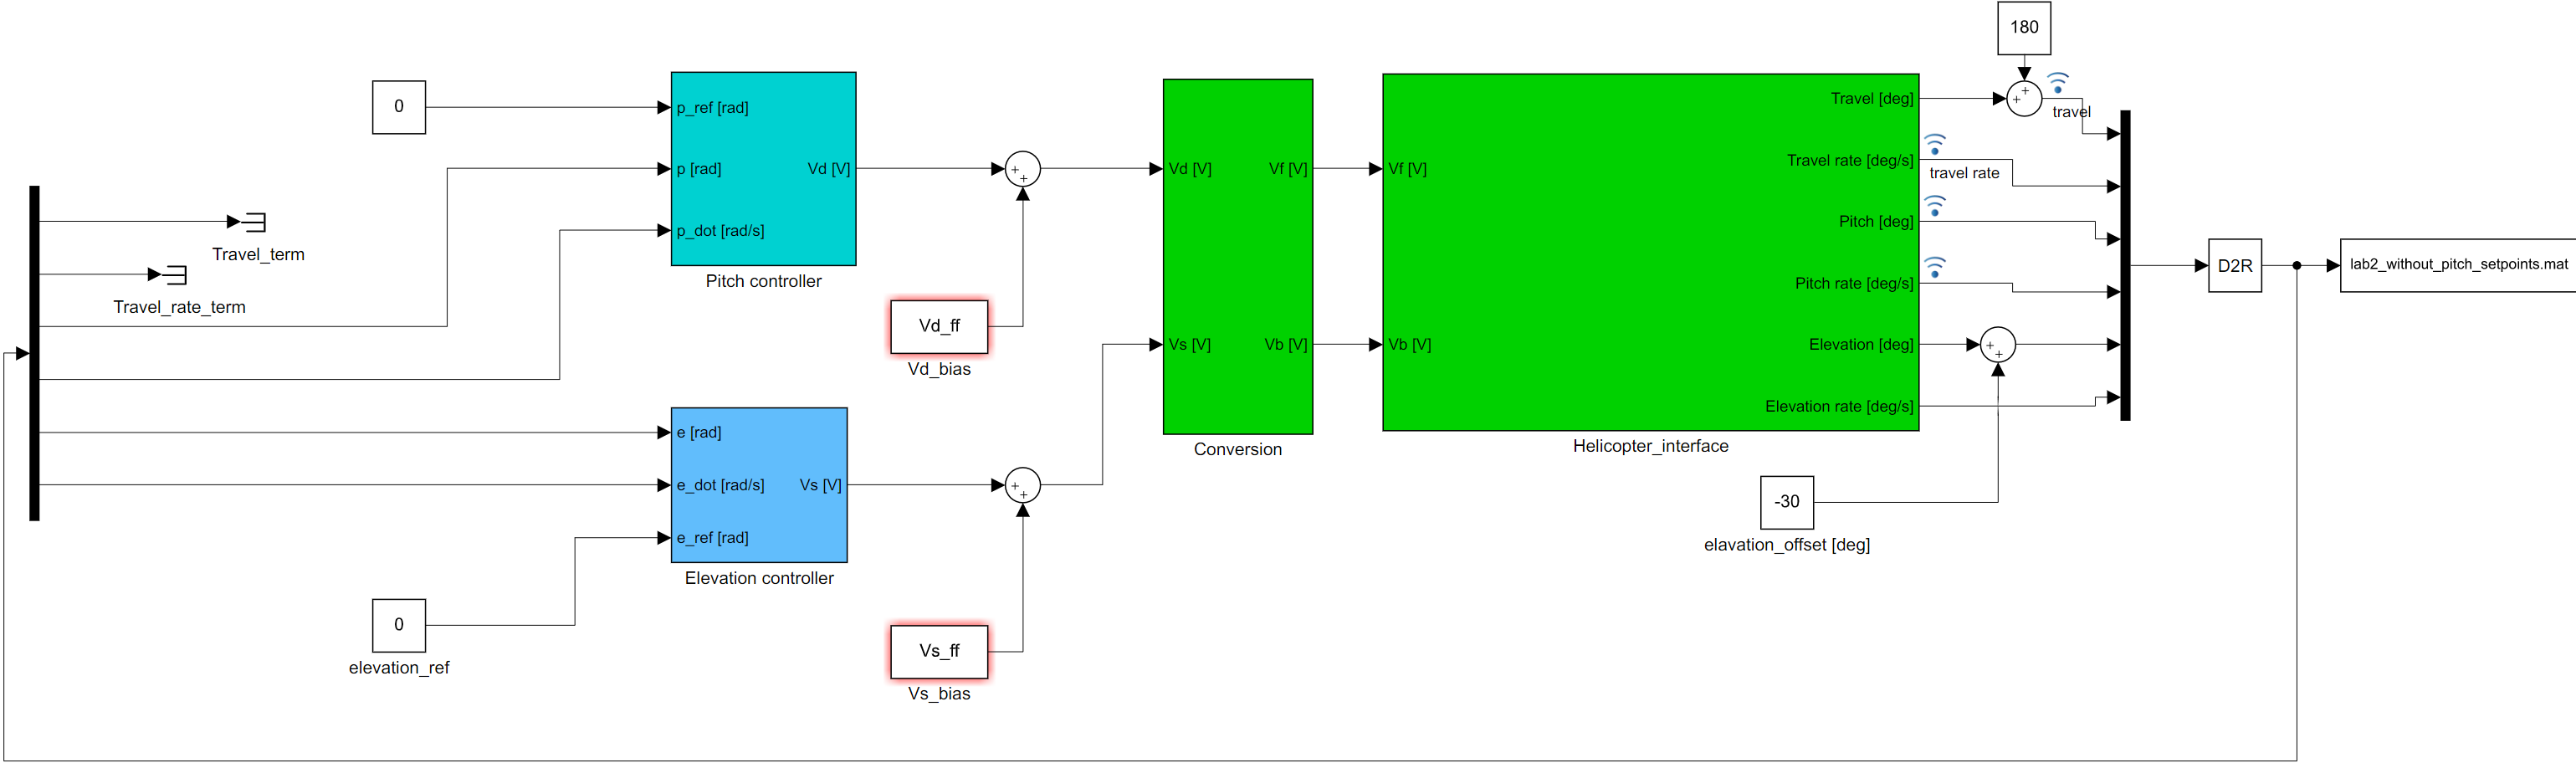
\includegraphics[angle=90, height=180mm]{code/lab2_simulink}
	\caption{Simulink diagram used in lab 2.}
	\label{fig:lab2_simulink}
\end{figure}
\end{document}